\chapter{Introducción}

En el presente trabajo se realiza el análisis estadístico de texto, empleando como fuente a los comentarios de la transmisión en vivo del primer debate presidencial, realizado el día 7 de abril del 2024; los comentarios presentan una estructura lingüística mal estructurada, de igual forma, se identifican Emojis entre apalabras o comentarios completos a partir de los mismos.\\


\section{Primer objetivo}
 Generar información estadística que nos permita visualizar los elementos característicos, que forman parte de los comentarios, como son, la frecuencia palabras, autores o usuarios con mas participación, votos a los comentarios (Top 10 de autores con mas votos), frecuencias de participación en los comentarios (Top 10 de autores con mas replicas) y la relación entre los votos y las replicas.\\

\section{Segundo objetivo}
 Realizar una comparativa entre el numero de menciones y la estadística de intención de voto previo a este debate, a modo de comparación estadística entre la expresión del nombre de los candidatos en los comentarios y la intención de voto documentada hasta ese momento.\\
   


\chapter{descripción de los datos}

Del total de datos unicamente consideraremos el siguiente conjunto de columnas:\\

\begin{itemize}
	\item ID: identificador de comentario
	\item text : Comentario del Usuario.
	\item author : Nombre de usuario que realiza el comentario.
	\item votes : numero de votos recibidos 
	\item replies : número de replicas en los comentarios.\\
\end{itemize} 

Se identifican un total de 1969 comentarios publicados en el video de Youtube (URL: https://www.youtube.com/watch?v=kZaucITWv00\&t=18s), un conteo total de datos de 18958, de los cuales destaca como Top la palabra claudia con un conteo de 419; continuación se muestra un ejemplo de los datos y su distribución.\\


\begin{table}[H]
	\centering
	\resizebox{\textwidth}{!}{%
		\begin{tabular}{ccccc}
			\rowcolor[HTML]{9B9B9B} 
			\textbf{ID}             & \textbf{text}                                      & \textbf{author}         & \textbf{votes}          & \textbf{replies}        \\
			0                       & El reloj debió verse en todo momento, para ten...  & @celinaramirez6363      & 394                     & 16.0                    \\
			1                       & Me uno a exigir que pongan los relojes de los ...  & @puellacodicum8569      & 555                     & 19.0                    \\
			2                       & Me parece muy bien cómo contestó Maynes, fue d...  & @alondrareal8518        & 79                      & NaN                     \\
			\multicolumn{1}{l}{...} & \multicolumn{1}{l}{...}                            & \multicolumn{1}{l}{...} & \multicolumn{1}{l}{...} & \multicolumn{1}{l}{...} \\
			1967                    & Salud puras citas tras citas así te la llevan ... & @mariacasildaramirezguzman9415       & 0                       & NaN                     \\
			1968                    & Claudia la mejor y vas a ser presidenta el pue...                                 & @tatianavazquez9617  & 0                       & NaN                     \\
			1969                    & Cuánto dinero les pagaste por esos reconocimie...  & @maru641                & 0                       & NaN                    
		\end{tabular}%
	}
	\caption{}
	\label{tab:T1}
\end{table}

A partir del conjunto de datos se generan estadísticos básicos referente a los datos de interés así como representaciones graficas de las distribuciones de los valores que resultan de interés.\\

 \section{Análisis estadístico básico}
 
 Del total los 1969 comentarios, se identifican 1214 usuarios de los cuales @DoloresMotaHernandez es la que presenta mayor participación, con un total de 27 comentarios en el video.\\
 
\begin{figure}[!h]
	\centering
	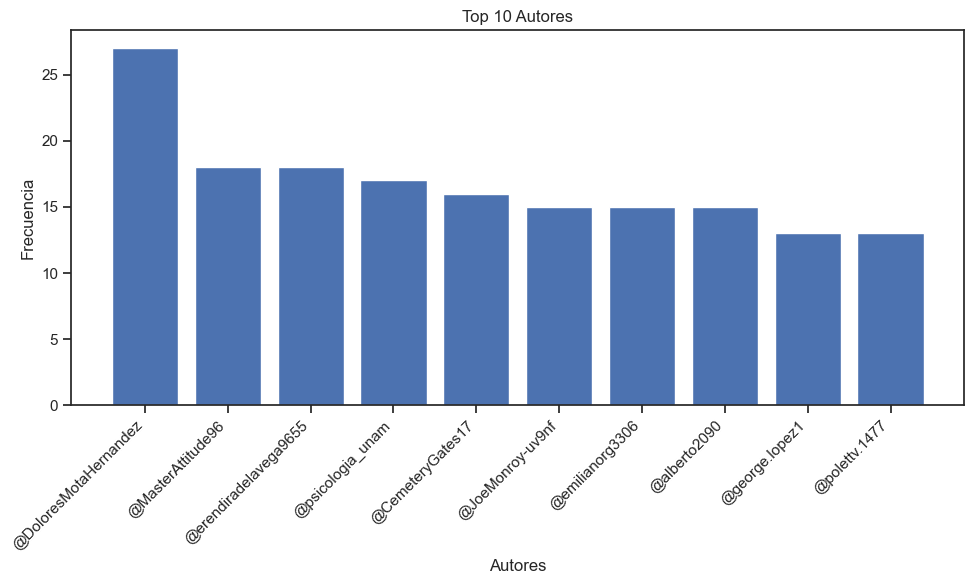
\includegraphics[width=15cm]{../Datos/top10autores}
	\caption{Top 10 de autores con más comentarios.}
	\label{fig:top10A}
\end{figure}

Si observamos el numero de votos con relación a los autores, la gran mayoría de los votos se concentran en pocos comentarios, como se puede observar en el top 10 de autores con más votos.\\

En cuanto a los datos estadísticos de los votos, podemos observar un conteo de 1021 comentarios con votos, de los cuales, el valor minimo corresponde a 1 voto,el 25\% 1 voto, el 50\% 4 voto, el 75\% 15 voto, presentando una menor distribución los valores mas altos de votos, se identifica el valor máximo a 1200 votos.\\

\begin{figure}[!h]
	\centering
	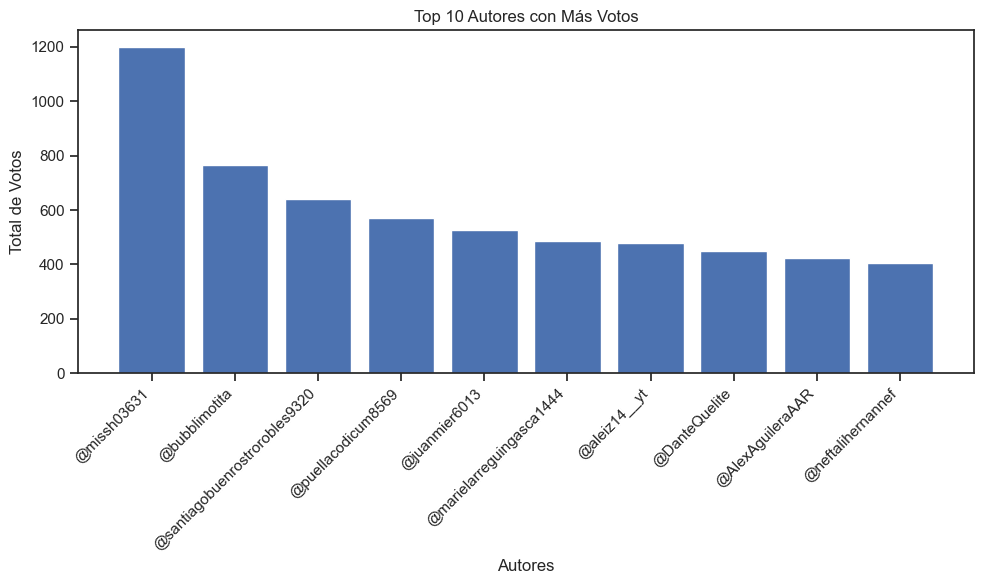
\includegraphics[width=15cm]{../Datos/top10autoresMasVotos}
	\caption{Top 10 de autores con comentarios más votados.}
	\label{fig:top10AMV}
\end{figure}

Podemos identificar un numero que solo un pequeño numero de comentarios recibieron replicas, es decir comentarios dentro de ellos. correspondiendo a 201 comentarios con replicas, ademas se observa una distribución menos dispersa en comparación con el numero de votos, se observa una media de 4.5 replicas, desviación estándar de 6.1, valor mínimo de 1, el 25\% con valor de 1, el 50\% con un valor de 2, el 75\% corresponde a 5 replicas y el valor máximo llega a 42 replicas.\\

\begin{figure}[!h]
	\centering
	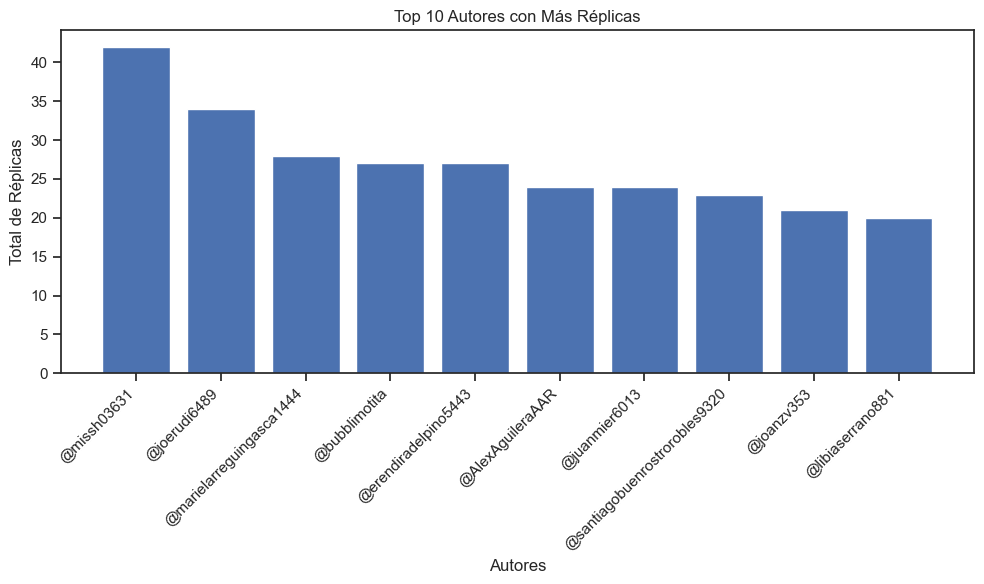
\includegraphics[width=15cm]{../Datos/top10autoresMasReplicas}
	\caption{Top 10 de comentarios de autores con mayor numero de replicas.}
	\label{fig:top10AMR}
\end{figure}

Al comparar la distribución de los votos contra las replicas, podemos notar una correlación entre aquellos mensajes que presentan un numero alto de votos y los que cuentan un con interacción en los comentarios , es decir un mayor numero de replicas, esto también se observa en las graficas anteriores donde podemos notar como algunos autores repiten en los Top.\\
  
\begin{figure}[!h]
	\centering
	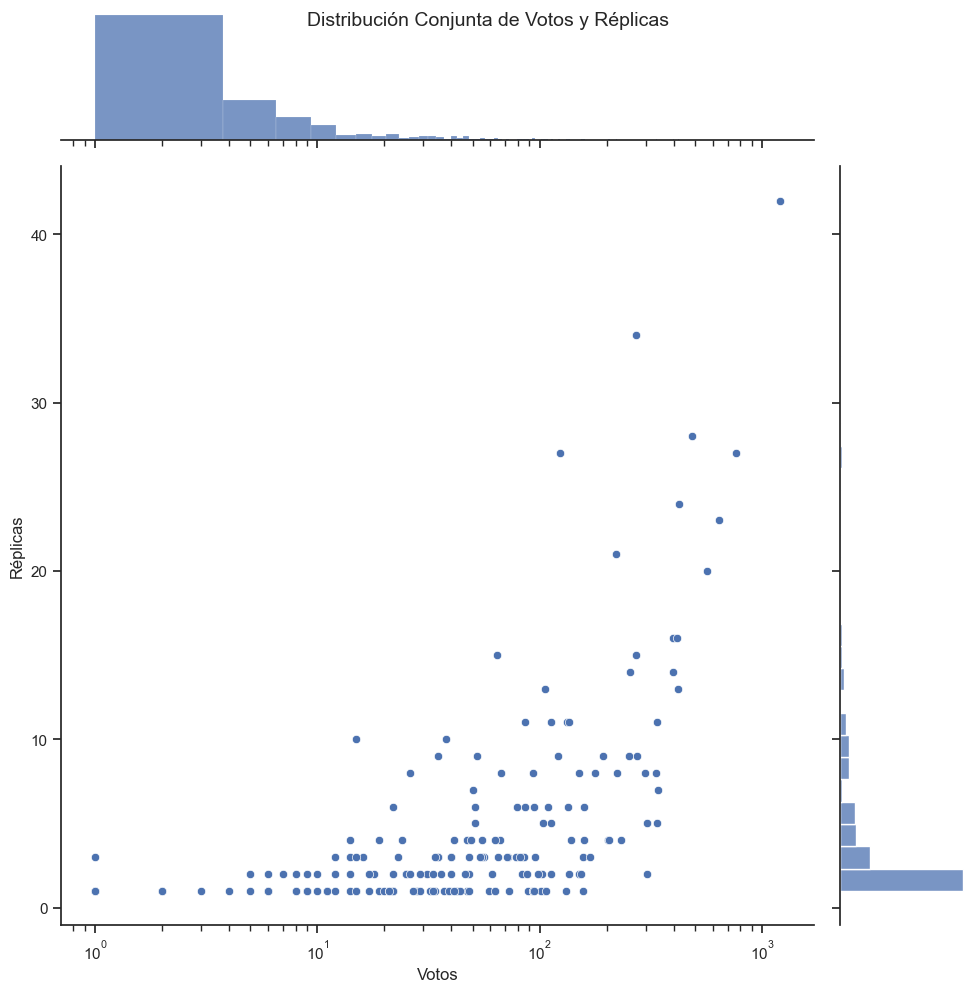
\includegraphics[width=15cm]{../Datos/DistribucionVotosVsReplicas}
	\caption{Top 10 de comentarios de autores con mayor numero de replicas.}
	\label{fig:DVVR}
\end{figure}

\chapter{Análisis de los comentarios}

Al realizar los estadísticos básicos en los comentarios podemos observar la distribución de las palabras mas recurrentes entre los comentarios, lo a partir de estos datos se genera el siguiente grafico, donde podemos observar la distribución del Top 20 de las palabras mas frecuentes destacando lo siguiente:\\

\begin{figure}[!h]
	\centering
	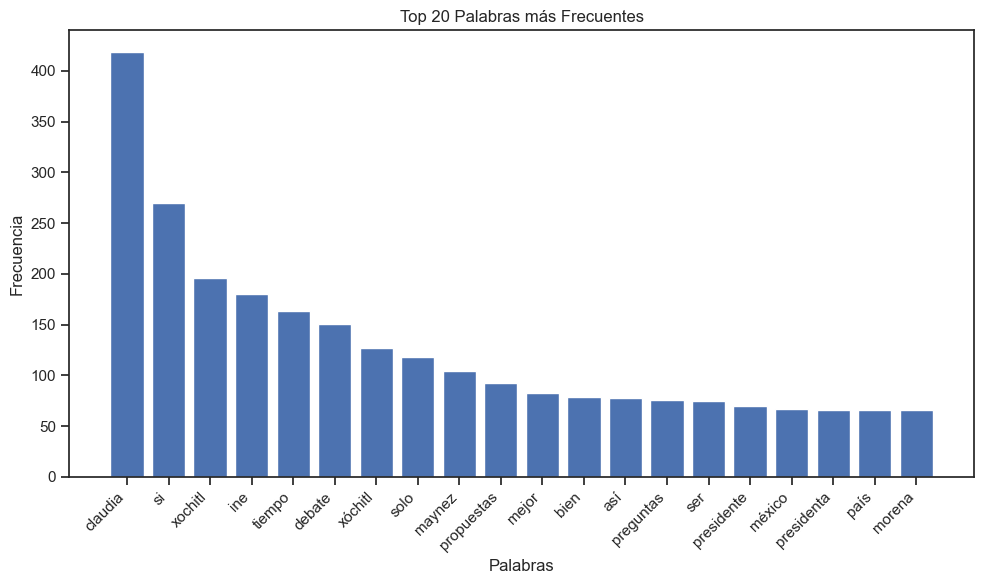
\includegraphics[width=16cm]{../Datos/top20palabrasMasFrecuentes}
	\caption{Top 10 de comentarios de autores con mayor numero de replicas.}
	\label{fig:Top20PMF}
\end{figure}

En el Top 20 podemos identificar los nombres de los candidatos que se presentaron en el primer debate, a los candidatos se busca relacionar las distintas formas como se les menciona, por lo que se busca homogenizar la escritura empleando filtrado y transformaciones, usando técnicas de stordswords, desidencias y stemmer a fin de concentrar palabras.\\

A la clasificación antes mencionada, se suman formas distintas de mencionar a los candidatos como son claudia, sheinbaum, xochitl, xóchitl, maynez, considerando estas menciones como apoyos directo a cada uno de los candidatos, sumando a su conteo total.\\

Como agregado se incluye la nuve de palabras mas frecuentes, de modo que el lector pueda observar de forma mas grafica las relevancia (frecuencia) de cada palabra y mencionada en los comentarios, lo que representa un mayor peso o interés publico.\\

\begin{figure}[!h]
	\centering
	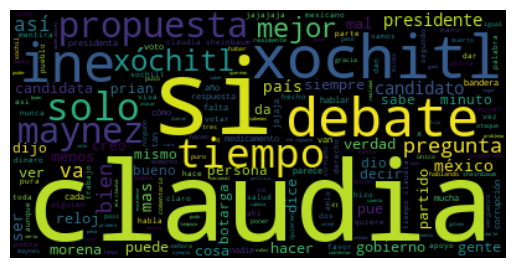
\includegraphics[width=16cm]{../Datos/NuveDePalabras}
	\caption{Top 10 de comentarios de autores con mayor numero de replicas.}
	\label{fig:NDP}
\end{figure}


\chapter{Conclusiones}

Según las encuestas y análisis publicados antes del primer debate presidencial en México 2024, las intenciones de voto se distribuían de la siguiente manera:\\

Claudia Sheinbaum (Morena, PT y PVEM): \textbf{49\%}; Xóchitl Gálvez (PRI-PAN-PRD): \textbf{26\%}; Jorge Álvarez Máynez (Movimiento Ciudadano): \textbf{18\%} (según encuesta “flash” publicada el 7 de abril de 2024)\\

La encuesta de El Financiero del 1 de abril de 2024 mostraba que Sheinbaum lideraba con un \textbf{35\%}, seguida de Gálvez con un \textbf{25\%} y Máynez con un \textbf{15\%}.\\


La encuesta de FactoMétrica y Reporte Índigo publicada el 9 de abril de 2024 mostraba que Sheinbaum lideraba con un \textbf{69\%}, seguida de Gálvez con un \textbf{26,5\%} y Máynez con un \textbf{4,5\%}.\\


La encuesta “flash” publicada el 7 de abril de 2024 mostraba que Sheinbaum lideraba con un \textbf{49\%}, seguida de Gálvez con un \textbf{26\%} y Máynez con un \textbf{18\%}.\\

Los resultados para los porcentajes de intención de voto los cuales los relacionamos con el apoyo en los comentarios, es decir, cada mención y sus variantes de cada candidato, quedan representados de la siguiente manera:\\

\begin{center}
	total de veces que se menciona el nombre de algún candidato:  \textbf{896}\\

Porcentaje de menciones de claudia-sheinbaum: \textbf{52.34\%}.\\

Porcentaje de menciones de xochitl-xóchitl: \textbf{36.05\%}.\\

Porcentaje de menciones de Maynez: \textbf{11.61\%.}

\end{center}

Como se puede observar si se identifica una similitud con la tendencia de intención de voto de las encuestadoras y el apoyo mostrado de la población interesada en un candidato, representado por comentarios o menciones de dicho candidato durante un evento publico en el que participan directamente los tres actores políticos.\\

Es posible medir el apoyo directamente por la cantidad de menciones en un debate en vivo, sin embargo la participación solo representa aun sector de la población que cuenta con internet, acceso a youtube mediante una cuenta, y cabe la posibilidad de que algunas participaciones sean Bots pagados.\\
